% Options for packages loaded elsewhere
\PassOptionsToPackage{unicode}{hyperref}
\PassOptionsToPackage{hyphens}{url}
\PassOptionsToPackage{dvipsnames,svgnames,x11names}{xcolor}
%
\documentclass[
  letterpaper,
  DIV=11,
  numbers=noendperiod]{scrartcl}

\usepackage{amsmath,amssymb}
\usepackage{iftex}
\ifPDFTeX
  \usepackage[T1]{fontenc}
  \usepackage[utf8]{inputenc}
  \usepackage{textcomp} % provide euro and other symbols
\else % if luatex or xetex
  \usepackage{unicode-math}
  \defaultfontfeatures{Scale=MatchLowercase}
  \defaultfontfeatures[\rmfamily]{Ligatures=TeX,Scale=1}
\fi
\usepackage{lmodern}
\ifPDFTeX\else  
    % xetex/luatex font selection
\fi
% Use upquote if available, for straight quotes in verbatim environments
\IfFileExists{upquote.sty}{\usepackage{upquote}}{}
\IfFileExists{microtype.sty}{% use microtype if available
  \usepackage[]{microtype}
  \UseMicrotypeSet[protrusion]{basicmath} % disable protrusion for tt fonts
}{}
\makeatletter
\@ifundefined{KOMAClassName}{% if non-KOMA class
  \IfFileExists{parskip.sty}{%
    \usepackage{parskip}
  }{% else
    \setlength{\parindent}{0pt}
    \setlength{\parskip}{6pt plus 2pt minus 1pt}}
}{% if KOMA class
  \KOMAoptions{parskip=half}}
\makeatother
\usepackage{xcolor}
\setlength{\emergencystretch}{3em} % prevent overfull lines
\setcounter{secnumdepth}{-\maxdimen} % remove section numbering
% Make \paragraph and \subparagraph free-standing
\makeatletter
\ifx\paragraph\undefined\else
  \let\oldparagraph\paragraph
  \renewcommand{\paragraph}{
    \@ifstar
      \xxxParagraphStar
      \xxxParagraphNoStar
  }
  \newcommand{\xxxParagraphStar}[1]{\oldparagraph*{#1}\mbox{}}
  \newcommand{\xxxParagraphNoStar}[1]{\oldparagraph{#1}\mbox{}}
\fi
\ifx\subparagraph\undefined\else
  \let\oldsubparagraph\subparagraph
  \renewcommand{\subparagraph}{
    \@ifstar
      \xxxSubParagraphStar
      \xxxSubParagraphNoStar
  }
  \newcommand{\xxxSubParagraphStar}[1]{\oldsubparagraph*{#1}\mbox{}}
  \newcommand{\xxxSubParagraphNoStar}[1]{\oldsubparagraph{#1}\mbox{}}
\fi
\makeatother

\usepackage{color}
\usepackage{fancyvrb}
\newcommand{\VerbBar}{|}
\newcommand{\VERB}{\Verb[commandchars=\\\{\}]}
\DefineVerbatimEnvironment{Highlighting}{Verbatim}{commandchars=\\\{\}}
% Add ',fontsize=\small' for more characters per line
\usepackage{framed}
\definecolor{shadecolor}{RGB}{241,243,245}
\newenvironment{Shaded}{\begin{snugshade}}{\end{snugshade}}
\newcommand{\AlertTok}[1]{\textcolor[rgb]{0.68,0.00,0.00}{#1}}
\newcommand{\AnnotationTok}[1]{\textcolor[rgb]{0.37,0.37,0.37}{#1}}
\newcommand{\AttributeTok}[1]{\textcolor[rgb]{0.40,0.45,0.13}{#1}}
\newcommand{\BaseNTok}[1]{\textcolor[rgb]{0.68,0.00,0.00}{#1}}
\newcommand{\BuiltInTok}[1]{\textcolor[rgb]{0.00,0.23,0.31}{#1}}
\newcommand{\CharTok}[1]{\textcolor[rgb]{0.13,0.47,0.30}{#1}}
\newcommand{\CommentTok}[1]{\textcolor[rgb]{0.37,0.37,0.37}{#1}}
\newcommand{\CommentVarTok}[1]{\textcolor[rgb]{0.37,0.37,0.37}{\textit{#1}}}
\newcommand{\ConstantTok}[1]{\textcolor[rgb]{0.56,0.35,0.01}{#1}}
\newcommand{\ControlFlowTok}[1]{\textcolor[rgb]{0.00,0.23,0.31}{\textbf{#1}}}
\newcommand{\DataTypeTok}[1]{\textcolor[rgb]{0.68,0.00,0.00}{#1}}
\newcommand{\DecValTok}[1]{\textcolor[rgb]{0.68,0.00,0.00}{#1}}
\newcommand{\DocumentationTok}[1]{\textcolor[rgb]{0.37,0.37,0.37}{\textit{#1}}}
\newcommand{\ErrorTok}[1]{\textcolor[rgb]{0.68,0.00,0.00}{#1}}
\newcommand{\ExtensionTok}[1]{\textcolor[rgb]{0.00,0.23,0.31}{#1}}
\newcommand{\FloatTok}[1]{\textcolor[rgb]{0.68,0.00,0.00}{#1}}
\newcommand{\FunctionTok}[1]{\textcolor[rgb]{0.28,0.35,0.67}{#1}}
\newcommand{\ImportTok}[1]{\textcolor[rgb]{0.00,0.46,0.62}{#1}}
\newcommand{\InformationTok}[1]{\textcolor[rgb]{0.37,0.37,0.37}{#1}}
\newcommand{\KeywordTok}[1]{\textcolor[rgb]{0.00,0.23,0.31}{\textbf{#1}}}
\newcommand{\NormalTok}[1]{\textcolor[rgb]{0.00,0.23,0.31}{#1}}
\newcommand{\OperatorTok}[1]{\textcolor[rgb]{0.37,0.37,0.37}{#1}}
\newcommand{\OtherTok}[1]{\textcolor[rgb]{0.00,0.23,0.31}{#1}}
\newcommand{\PreprocessorTok}[1]{\textcolor[rgb]{0.68,0.00,0.00}{#1}}
\newcommand{\RegionMarkerTok}[1]{\textcolor[rgb]{0.00,0.23,0.31}{#1}}
\newcommand{\SpecialCharTok}[1]{\textcolor[rgb]{0.37,0.37,0.37}{#1}}
\newcommand{\SpecialStringTok}[1]{\textcolor[rgb]{0.13,0.47,0.30}{#1}}
\newcommand{\StringTok}[1]{\textcolor[rgb]{0.13,0.47,0.30}{#1}}
\newcommand{\VariableTok}[1]{\textcolor[rgb]{0.07,0.07,0.07}{#1}}
\newcommand{\VerbatimStringTok}[1]{\textcolor[rgb]{0.13,0.47,0.30}{#1}}
\newcommand{\WarningTok}[1]{\textcolor[rgb]{0.37,0.37,0.37}{\textit{#1}}}

\providecommand{\tightlist}{%
  \setlength{\itemsep}{0pt}\setlength{\parskip}{0pt}}\usepackage{longtable,booktabs,array}
\usepackage{calc} % for calculating minipage widths
% Correct order of tables after \paragraph or \subparagraph
\usepackage{etoolbox}
\makeatletter
\patchcmd\longtable{\par}{\if@noskipsec\mbox{}\fi\par}{}{}
\makeatother
% Allow footnotes in longtable head/foot
\IfFileExists{footnotehyper.sty}{\usepackage{footnotehyper}}{\usepackage{footnote}}
\makesavenoteenv{longtable}
\usepackage{graphicx}
\makeatletter
\def\maxwidth{\ifdim\Gin@nat@width>\linewidth\linewidth\else\Gin@nat@width\fi}
\def\maxheight{\ifdim\Gin@nat@height>\textheight\textheight\else\Gin@nat@height\fi}
\makeatother
% Scale images if necessary, so that they will not overflow the page
% margins by default, and it is still possible to overwrite the defaults
% using explicit options in \includegraphics[width, height, ...]{}
\setkeys{Gin}{width=\maxwidth,height=\maxheight,keepaspectratio}
% Set default figure placement to htbp
\makeatletter
\def\fps@figure{htbp}
\makeatother

\KOMAoption{captions}{tableheading}
\makeatletter
\@ifpackageloaded{caption}{}{\usepackage{caption}}
\AtBeginDocument{%
\ifdefined\contentsname
  \renewcommand*\contentsname{Table of contents}
\else
  \newcommand\contentsname{Table of contents}
\fi
\ifdefined\listfigurename
  \renewcommand*\listfigurename{List of Figures}
\else
  \newcommand\listfigurename{List of Figures}
\fi
\ifdefined\listtablename
  \renewcommand*\listtablename{List of Tables}
\else
  \newcommand\listtablename{List of Tables}
\fi
\ifdefined\figurename
  \renewcommand*\figurename{Figure}
\else
  \newcommand\figurename{Figure}
\fi
\ifdefined\tablename
  \renewcommand*\tablename{Table}
\else
  \newcommand\tablename{Table}
\fi
}
\@ifpackageloaded{float}{}{\usepackage{float}}
\floatstyle{ruled}
\@ifundefined{c@chapter}{\newfloat{codelisting}{h}{lop}}{\newfloat{codelisting}{h}{lop}[chapter]}
\floatname{codelisting}{Listing}
\newcommand*\listoflistings{\listof{codelisting}{List of Listings}}
\makeatother
\makeatletter
\makeatother
\makeatletter
\@ifpackageloaded{caption}{}{\usepackage{caption}}
\@ifpackageloaded{subcaption}{}{\usepackage{subcaption}}
\makeatother

\ifLuaTeX
  \usepackage{selnolig}  % disable illegal ligatures
\fi
\usepackage{bookmark}

\IfFileExists{xurl.sty}{\usepackage{xurl}}{} % add URL line breaks if available
\urlstyle{same} % disable monospaced font for URLs
\hypersetup{
  pdftitle={Gaussian Process Simulation and Inference},
  colorlinks=true,
  linkcolor={blue},
  filecolor={Maroon},
  citecolor={Blue},
  urlcolor={Blue},
  pdfcreator={LaTeX via pandoc}}


\title{Gaussian Process Simulation and Inference}
\author{}
\date{}

\begin{document}
\maketitle


\subsection{Gaussian Process
Framework}\label{gaussian-process-framework}

A \textbf{Gaussian Process (GP)} is a distribution over functions such
that any finite collection of function values follows a multivariate
normal distribution:

{[} f(x) \sim \mathcal{GP}(m(x), k(x, x')). {]}

Here (m(x)) is the mean function and (k(x, x')) the covariance (kernel)
function.

\begin{Shaded}
\begin{Highlighting}[]
\FunctionTok{set.seed}\NormalTok{(}\DecValTok{120}\NormalTok{)}
\FunctionTok{suppressPackageStartupMessages}\NormalTok{(\{}
  \ControlFlowTok{if}\NormalTok{ (}\SpecialCharTok{!}\FunctionTok{requireNamespace}\NormalTok{(}\StringTok{"mvtnorm"}\NormalTok{, }\AttributeTok{quietly =} \ConstantTok{TRUE}\NormalTok{)) }\FunctionTok{install.packages}\NormalTok{(}\StringTok{"mvtnorm"}\NormalTok{)}
  \ControlFlowTok{if}\NormalTok{ (}\SpecialCharTok{!}\FunctionTok{requireNamespace}\NormalTok{(}\StringTok{"ggplot2"}\NormalTok{, }\AttributeTok{quietly =} \ConstantTok{TRUE}\NormalTok{)) }\FunctionTok{install.packages}\NormalTok{(}\StringTok{"ggplot2"}\NormalTok{)}
\NormalTok{\})}
\FunctionTok{library}\NormalTok{(mvtnorm)}
\end{Highlighting}
\end{Shaded}

\begin{verbatim}
Warning: package 'mvtnorm' was built under R version 4.4.3
\end{verbatim}

\begin{Shaded}
\begin{Highlighting}[]
\FunctionTok{library}\NormalTok{(ggplot2)}
\end{Highlighting}
\end{Shaded}

\begin{verbatim}
Warning: package 'ggplot2' was built under R version 4.4.3
\end{verbatim}

\begin{Shaded}
\begin{Highlighting}[]
\CommentTok{\# Helper: squared Euclidean distance for 1D vectors}
\NormalTok{sqdist }\OtherTok{\textless{}{-}} \ControlFlowTok{function}\NormalTok{(x, xprime) \{}
  \FunctionTok{outer}\NormalTok{(x, xprime, }\ControlFlowTok{function}\NormalTok{(a, b) (a }\SpecialCharTok{{-}}\NormalTok{ b)}\SpecialCharTok{\^{}}\DecValTok{2}\NormalTok{)}
\NormalTok{\}}

\CommentTok{\# Exponentiated quadratic (RBF) kernel = Stan\textquotesingle{}s cov\_exp\_quad(alpha, rho)}
\CommentTok{\# K\_ij = alpha\^{}2 * exp( {-}0.5 * (x\_i {-} x\_j)\^{}2 / rho\^{}2 )}
\NormalTok{cov\_exp\_quad }\OtherTok{\textless{}{-}} \ControlFlowTok{function}\NormalTok{(x, xprime, alpha, rho) \{}
\NormalTok{  alpha}\SpecialCharTok{\^{}}\DecValTok{2} \SpecialCharTok{*} \FunctionTok{exp}\NormalTok{(}\SpecialCharTok{{-}}\FloatTok{0.5} \SpecialCharTok{*} \FunctionTok{sqdist}\NormalTok{(x, xprime) }\SpecialCharTok{/}\NormalTok{ (rho}\SpecialCharTok{\^{}}\DecValTok{2}\NormalTok{))}
\NormalTok{\}}

\CommentTok{\# Tiny jitter (nugget) for numerical stability (same idea as tutorial\textquotesingle{}s 1e{-}10)}
\NormalTok{jitter\_eps }\OtherTok{\textless{}{-}} \FloatTok{1e{-}10}
\end{Highlighting}
\end{Shaded}

\subsection{GP Prior Simulation}\label{gp-prior-simulation}

We adopt the \textbf{squared exponential (RBF) kernel}:

{[} k(x\_i, x\_j) = \alpha\^{}2
\exp!\left(-\frac{(x_i - x_j)^2}{2 \rho^2}\right), {]}

with hyperparameters: - (\alpha): marginal standard deviation (vertical
variability), - (\rho): length-scale (smoothness).

Given a grid of inputs (\mathbf{x} = (x\_1,\dots,x\_n)), the prior is

{[} \mathbf{f} \sim \mathcal{N}!\big( \mathbf{0},
K(\mathbf{x},\mathbf{x}) + \epsilon I \big), {]}

where (K) is the Gram matrix of kernel evaluations and (\epsilon) is a
small jitter term.

\begin{Shaded}
\begin{Highlighting}[]
\CommentTok{\# Simulate from a GP prior}

\CommentTok{\#Grid}
\NormalTok{N  }\OtherTok{\textless{}{-}} \DecValTok{551}
\NormalTok{x  }\OtherTok{\textless{}{-}} \DecValTok{22} \SpecialCharTok{*}\NormalTok{ (}\DecValTok{0}\SpecialCharTok{:}\NormalTok{(N }\SpecialCharTok{{-}} \DecValTok{1}\NormalTok{)) }\SpecialCharTok{/}\NormalTok{ (N }\SpecialCharTok{{-}} \DecValTok{1}\NormalTok{) }\SpecialCharTok{{-}} \DecValTok{11}

\CommentTok{\# GP hyperparameters }
\NormalTok{alpha\_true }\OtherTok{\textless{}{-}} \DecValTok{3}
\NormalTok{rho\_true   }\OtherTok{\textless{}{-}} \FloatTok{5.5}

\CommentTok{\# Prior covariance on the grid + jitter}
\NormalTok{K\_xx }\OtherTok{\textless{}{-}} \FunctionTok{cov\_exp\_quad}\NormalTok{(x, x, alpha\_true, rho\_true) }\SpecialCharTok{+} \FunctionTok{diag}\NormalTok{(jitter\_eps, N)}

\CommentTok{\# Draw ONE prior sample f \textasciitilde{} N(0, K\_xx)}
\NormalTok{f\_prior }\OtherTok{\textless{}{-}} \FunctionTok{as.numeric}\NormalTok{(}\FunctionTok{rmvnorm}\NormalTok{(}\DecValTok{1}\NormalTok{, }\AttributeTok{mean =} \FunctionTok{rep}\NormalTok{(}\DecValTok{0}\NormalTok{, N), }\AttributeTok{sigma =}\NormalTok{ K\_xx))}
\CommentTok{\#One draw}
\FunctionTok{qplot}\NormalTok{(x, f\_prior, }\AttributeTok{geom =} \StringTok{"line"}\NormalTok{) }\SpecialCharTok{+}
  \FunctionTok{labs}\NormalTok{(}\AttributeTok{title =} \StringTok{"One GP prior draw"}\NormalTok{, }\AttributeTok{x =} \StringTok{"x"}\NormalTok{, }\AttributeTok{y =} \StringTok{"f(x)"}\NormalTok{)}
\end{Highlighting}
\end{Shaded}

\begin{verbatim}
Warning: `qplot()` was deprecated in ggplot2 3.4.0.
\end{verbatim}

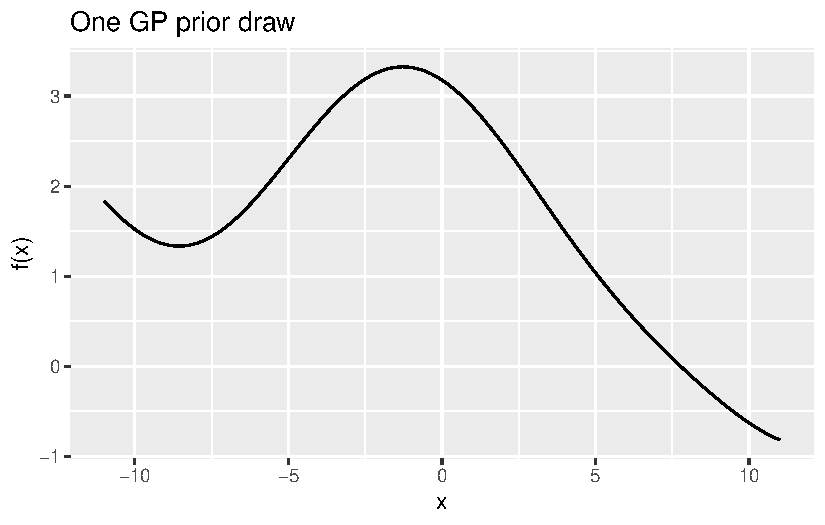
\includegraphics{GP-simulation-+-inference_files/figure-pdf/unnamed-chunk-2-1.pdf}

\subsection{Observational Model}\label{observational-model}

We assume noisy Gaussian observations:

{[} y\_i \sim \mathcal{N}(f(x\_i), \sigma\^{}2), {]}

with (\sigma\^{}2) denoting measurement noise variance.

\begin{Shaded}
\begin{Highlighting}[]
\CommentTok{\#  Simulate data with a Gaussian likelihood }

\NormalTok{sigma\_true }\OtherTok{\textless{}{-}} \DecValTok{2}  \CommentTok{\# observation noise sd}
\CommentTok{\# We\textquotesingle{}ll "observe" only 11 evenly spaced points on the grid }
\NormalTok{obs\_idx }\OtherTok{\textless{}{-}} \DecValTok{50} \SpecialCharTok{*}\NormalTok{ (}\DecValTok{0}\SpecialCharTok{:}\DecValTok{10}\NormalTok{) }\SpecialCharTok{+} \DecValTok{26}   \CommentTok{\# 11 indices spread across x}
\NormalTok{x\_obs   }\OtherTok{\textless{}{-}}\NormalTok{ x[obs\_idx]}
\NormalTok{f\_obs   }\OtherTok{\textless{}{-}}\NormalTok{ f\_prior[obs\_idx]}
\NormalTok{y\_obs   }\OtherTok{\textless{}{-}}\NormalTok{ f\_obs }\SpecialCharTok{+} \FunctionTok{rnorm}\NormalTok{(}\FunctionTok{length}\NormalTok{(obs\_idx), }\DecValTok{0}\NormalTok{, sigma\_true)}

\CommentTok{\# Plot: prior draw (thin) + noisy observations (points)}
\NormalTok{df\_all }\OtherTok{\textless{}{-}} \FunctionTok{data.frame}\NormalTok{(}\AttributeTok{x =}\NormalTok{ x, }\AttributeTok{f =}\NormalTok{ f\_prior)}
\NormalTok{df\_obs }\OtherTok{\textless{}{-}} \FunctionTok{data.frame}\NormalTok{(}\AttributeTok{x =}\NormalTok{ x\_obs, }\AttributeTok{y =}\NormalTok{ y\_obs)}
\FunctionTok{ggplot}\NormalTok{() }\SpecialCharTok{+}
  \FunctionTok{geom\_line}\NormalTok{(}\AttributeTok{data =}\NormalTok{ df\_all, }\FunctionTok{aes}\NormalTok{(x, f), }\AttributeTok{linewidth =} \FloatTok{0.6}\NormalTok{) }\SpecialCharTok{+}
  \FunctionTok{geom\_point}\NormalTok{(}\AttributeTok{data =}\NormalTok{ df\_obs, }\FunctionTok{aes}\NormalTok{(x, y), }\AttributeTok{size =} \DecValTok{2}\NormalTok{) }\SpecialCharTok{+}
  \FunctionTok{labs}\NormalTok{(}\AttributeTok{title =} \StringTok{"Noisy observations from GP + Gaussian noise"}\NormalTok{,}
       \AttributeTok{x =} \StringTok{"x"}\NormalTok{, }\AttributeTok{y =} \StringTok{"y"}\NormalTok{)}
\end{Highlighting}
\end{Shaded}

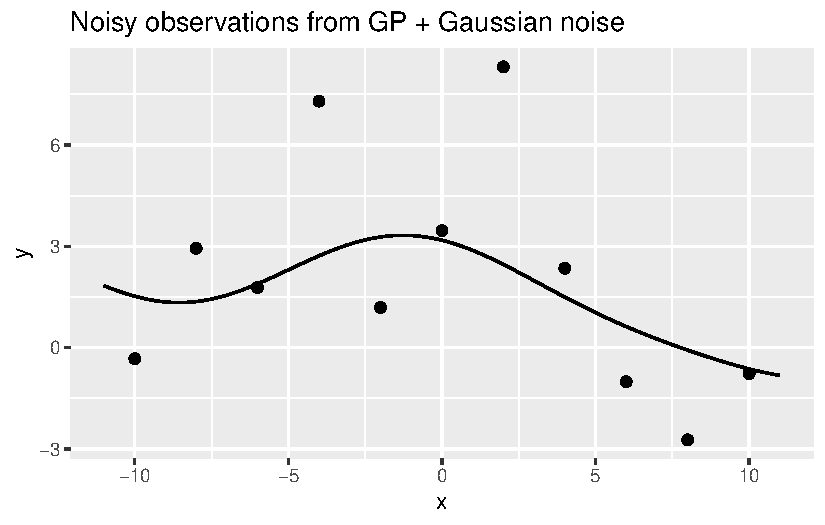
\includegraphics{GP-simulation-+-inference_files/figure-pdf/unnamed-chunk-3-1.pdf}

\begin{Shaded}
\begin{Highlighting}[]
\CommentTok{\# Fit GP regression analytically (Sec. 2.4)}
\CommentTok{\#     (Posterior of f\_* | y with Gaussian noise)}

\CommentTok{\# Build the cross{-}covariances}
\NormalTok{K\_oo }\OtherTok{\textless{}{-}} \FunctionTok{cov\_exp\_quad}\NormalTok{(x\_obs, x\_obs, alpha\_true, rho\_true) }\SpecialCharTok{+} \FunctionTok{diag}\NormalTok{(sigma\_true}\SpecialCharTok{\^{}}\DecValTok{2}\NormalTok{, }\FunctionTok{length}\NormalTok{(obs\_idx))}
\NormalTok{K\_po }\OtherTok{\textless{}{-}} \FunctionTok{cov\_exp\_quad}\NormalTok{(x, x\_obs, alpha\_true, rho\_true)   }\CommentTok{\# pred x obs}
\NormalTok{K\_pp }\OtherTok{\textless{}{-}} \FunctionTok{cov\_exp\_quad}\NormalTok{(x, x, alpha\_true, rho\_true)       }\CommentTok{\# pred x pred}

\CommentTok{\# Solve with Cholesky instead of inverting (stable \& fast)}
\NormalTok{L\_oo }\OtherTok{\textless{}{-}} \FunctionTok{chol}\NormalTok{(K\_oo)                                     }\CommentTok{\# K\_oo = L L\^{}T}
\NormalTok{alpha\_vec }\OtherTok{\textless{}{-}} \FunctionTok{backsolve}\NormalTok{(L\_oo, }\FunctionTok{forwardsolve}\NormalTok{(L\_oo, y\_obs, }\AttributeTok{upper.tri =} \ConstantTok{TRUE}\NormalTok{, }\AttributeTok{transpose =} \ConstantTok{TRUE}\NormalTok{))}

\CommentTok{\# Posterior mean: mu = K\_* K\_oo\^{}\{{-}1\} y}
\NormalTok{post\_mu }\OtherTok{\textless{}{-}}\NormalTok{ K\_po }\SpecialCharTok{\%*\%}\NormalTok{ alpha\_vec}

\CommentTok{\# Posterior cov:  Sigma = K\_** {-} K\_* K\_oo\^{}\{{-}1\} K\_*\^{}T}
\CommentTok{\# Compute V = L\^{}\{{-}1\} K\_*\^{}T  (solve triangular systems)}
\NormalTok{V }\OtherTok{\textless{}{-}} \FunctionTok{backsolve}\NormalTok{(L\_oo, }\FunctionTok{t}\NormalTok{(K\_po), }\AttributeTok{upper.tri =} \ConstantTok{TRUE}\NormalTok{, }\AttributeTok{transpose =} \ConstantTok{TRUE}\NormalTok{)}
\NormalTok{post\_cov }\OtherTok{\textless{}{-}}\NormalTok{ K\_pp }\SpecialCharTok{{-}} \FunctionTok{t}\NormalTok{(V) }\SpecialCharTok{\%*\%}\NormalTok{ V}

\CommentTok{\# Draw posterior functions if you want spaghetti:}
\FunctionTok{set.seed}\NormalTok{(}\DecValTok{123}\NormalTok{)}
\NormalTok{n\_draw }\OtherTok{\textless{}{-}} \DecValTok{50}
\NormalTok{f\_post\_draws }\OtherTok{\textless{}{-}} \FunctionTok{rmvnorm}\NormalTok{(n\_draw, }\AttributeTok{mean =} \FunctionTok{as.numeric}\NormalTok{(post\_mu), }\AttributeTok{sigma =}\NormalTok{ post\_cov)}

\CommentTok{\# Plot: posterior mean +/{-} 2sd, plus points}
\NormalTok{post\_sd }\OtherTok{\textless{}{-}} \FunctionTok{sqrt}\NormalTok{(}\FunctionTok{diag}\NormalTok{(post\_cov))}
\NormalTok{df\_post }\OtherTok{\textless{}{-}} \FunctionTok{data.frame}\NormalTok{(}\AttributeTok{x =}\NormalTok{ x, }\AttributeTok{mu =} \FunctionTok{as.numeric}\NormalTok{(post\_mu), }\AttributeTok{lo =}\NormalTok{ post\_mu }\SpecialCharTok{{-}} \DecValTok{2}\SpecialCharTok{*}\NormalTok{post\_sd, }\AttributeTok{hi =}\NormalTok{ post\_mu }\SpecialCharTok{+} \DecValTok{2}\SpecialCharTok{*}\NormalTok{post\_sd)}

\FunctionTok{ggplot}\NormalTok{() }\SpecialCharTok{+}
  \FunctionTok{geom\_ribbon}\NormalTok{(}\AttributeTok{data =}\NormalTok{ df\_post, }\FunctionTok{aes}\NormalTok{(x, }\AttributeTok{ymin =}\NormalTok{ lo, }\AttributeTok{ymax =}\NormalTok{ hi), }\AttributeTok{alpha =} \FloatTok{0.2}\NormalTok{) }\SpecialCharTok{+}
  \FunctionTok{geom\_line}\NormalTok{(}\AttributeTok{data =}\NormalTok{ df\_post, }\FunctionTok{aes}\NormalTok{(x, }\AttributeTok{y =}\NormalTok{ mu), }\AttributeTok{linewidth =} \FloatTok{0.8}\NormalTok{) }\SpecialCharTok{+}
  \FunctionTok{geom\_point}\NormalTok{(}\AttributeTok{data =}\NormalTok{ df\_obs, }\FunctionTok{aes}\NormalTok{(x, y), }\AttributeTok{size =} \DecValTok{2}\NormalTok{) }\SpecialCharTok{+}
  \FunctionTok{labs}\NormalTok{(}\AttributeTok{title =} \StringTok{"Analytic GP posterior (mean ± 2sd)"}\NormalTok{,}
       \AttributeTok{x =} \StringTok{"x"}\NormalTok{, }\AttributeTok{y =} \StringTok{"f(x)"}\NormalTok{)}
\end{Highlighting}
\end{Shaded}

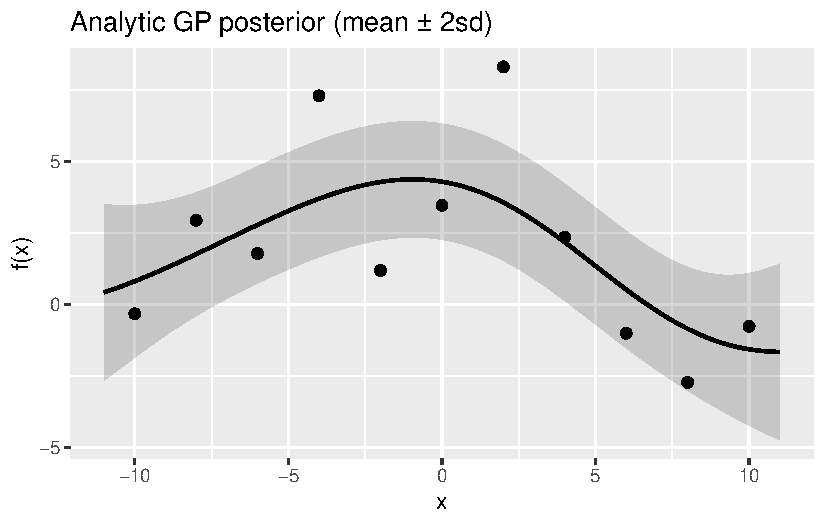
\includegraphics{GP-simulation-+-inference_files/figure-pdf/unnamed-chunk-4-1.pdf}

\begin{Shaded}
\begin{Highlighting}[]
\CommentTok{\# Spaghetti: overlay posterior function draws}
\NormalTok{draw\_df }\OtherTok{\textless{}{-}} \FunctionTok{data.frame}\NormalTok{(}\AttributeTok{x =} \FunctionTok{rep}\NormalTok{(x, n\_draw),}
                      \AttributeTok{f =} \FunctionTok{as.vector}\NormalTok{(}\FunctionTok{t}\NormalTok{(f\_post\_draws)),}
                      \AttributeTok{draw =} \FunctionTok{factor}\NormalTok{(}\FunctionTok{rep}\NormalTok{(}\DecValTok{1}\SpecialCharTok{:}\NormalTok{n\_draw, }\AttributeTok{each =} \FunctionTok{length}\NormalTok{(x))))}

\FunctionTok{ggplot}\NormalTok{(draw\_df, }\FunctionTok{aes}\NormalTok{(x, f, }\AttributeTok{group =}\NormalTok{ draw)) }\SpecialCharTok{+}
  \FunctionTok{geom\_line}\NormalTok{(}\AttributeTok{alpha =} \FloatTok{0.35}\NormalTok{) }\SpecialCharTok{+}
  \FunctionTok{geom\_point}\NormalTok{(}\AttributeTok{data =}\NormalTok{ df\_obs, }\FunctionTok{aes}\NormalTok{(x, y), }\AttributeTok{inherit.aes =} \ConstantTok{FALSE}\NormalTok{, }\AttributeTok{size =} \DecValTok{2}\NormalTok{) }\SpecialCharTok{+}
  \FunctionTok{labs}\NormalTok{(}\AttributeTok{title =} \StringTok{"Posterior draws (\textquotesingle{}spaghetti\textquotesingle{}) + observations"}\NormalTok{,}
       \AttributeTok{x =} \StringTok{"x"}\NormalTok{, }\AttributeTok{y =} \StringTok{"f(x)"}\NormalTok{)}
\end{Highlighting}
\end{Shaded}

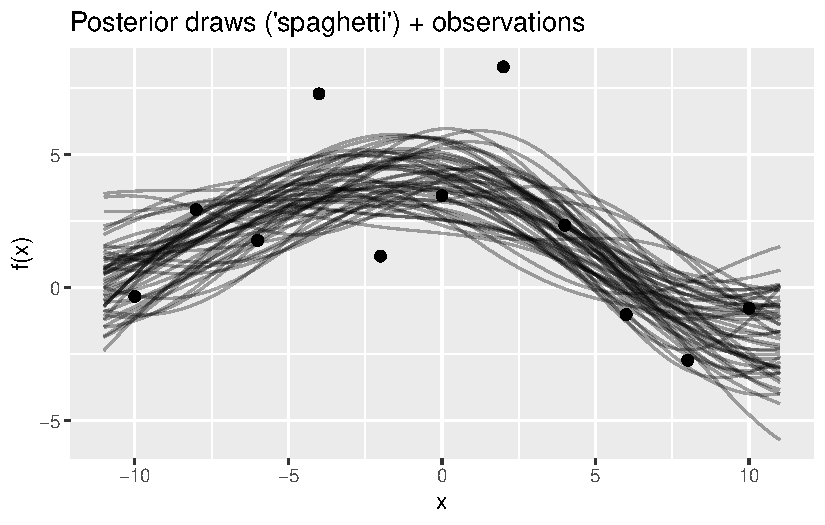
\includegraphics{GP-simulation-+-inference_files/figure-pdf/unnamed-chunk-5-1.pdf}

\subsection{Posterior Conditioning}\label{posterior-conditioning}

Conditioning on observed data ((\mathbf{x}\emph{\{obs\},
\mathbf{y}}\{obs\})), the posterior distribution at new points
(\mathbf{x}\_*) is Gaussian:

{[} \mathbf{f}\emph{* \mid \mathbf{y}}\{obs\} \sim  \mathcal{N}(\mu\_*,
\Sigma\_*), {]}

where

{[} \mu\emph{* = K(\mathbf{x}}*, \mathbf{x}\emph{\{obs\})
\big[ K(\mathbf{x}_{obs}, \mathbf{x}_{obs}) + \sigma^2 I \big]\^{}\{-1\}
\mathbf{y}}\{obs\}, {]}

{[} \Sigma\emph{* = K(\mathbf{x}}*, \mathbf{x}\_*) - K(\mathbf{x}\_*,
\mathbf{x}\emph{\{obs\})
\big[ K(\mathbf{x}_{obs}, \mathbf{x}_{obs}) + \sigma^2 I \big]\^{}\{-1\}
K(\mathbf{x}}\{obs\}, \mathbf{x}\_*). {]}

This yields closed-form inference without MCMC.




\end{document}
